% ----------------------------------------------------------------------
% ----------------------------------------------------------------------
\section*{Quantisierung}
Unter \emph{Quantisierung} (auch \emph{Diskretisierung}) versteht man die Unterteilung eines kontinuierlichen Raums in diskrete Abschnitte.

Indem man der reellen Zahl $2.71828$ beispielsweise alle Nachkommastellen entfernt, könnte man diese Zahl der natürlichen Zahl $2$ zuweisen. Hierbei ist klar, dass jede andere Zahl mit einer $2$ vor dem Komma ebenfalls der natürlichen Zahl $2$ zugewiesen würde. Die $2$ wäre also eine Art \emph{Repräsentant} für alle reellen Zahlen im Intervall $[2; 3)$.

Zu beachten ist, dass wir einen Raum auch unregelmäßig quantisieren können: So wäre der Zeitstrahl einer Woche beispielsweise in Arbeitstage und Wochenende quantisierbar.

\subsection*{Spezialfall: Digitalisierung}
Ein Spezialfall der Quantisierung ist die Digitalisierung: Im Fall der Digitalisierung sprechen wir immer von einer gleich"-mäßigen Quantisierung eines kontinuierlichen Raums in ein Zahlensystem zu einer bestimmten Basis.



% ----------------------------------------------------------------------
% ----------------------------------------------------------------------
\section*{Idee von LVQ}
LVQ beschreibt eine Gruppe von \emph{überwachten} Lernalgorithmen (LVQ1, LVQ2, LVQ3 und OLVQ) und basiert auf der Vektorquantisierung (VQ), einem unüberwachten Clustering- und Lernalgorithmus.

\subsection*{Vektorquantisierung (VQ)}
Ziel der Vektorquantisierung ist es, den Merkmalsraum mit einer geringen Anzahl an Vektoren zu approximieren.
Hierfür wird eine Menge von Merkmalsvektoren $x$ zu $M$ Klassen zugeordnet. Jede dieser Klassen hat einen \emph{Prototypvektor}. Die Menge aller Prototypvektoren wird als \emph{Codebook} bezeichnet (weshalb die Prototypvektoren auch als Codebookvektoren bezeichnet werden).
Ein Merkmalsvektor $x$ wird derjenigen Klasse zugeordnet, zu welcher der Abstand zwischen Merkmalsvektor und Prototypvektor am kleinsten ist.

\begin{figure}[ht!] \centering 
	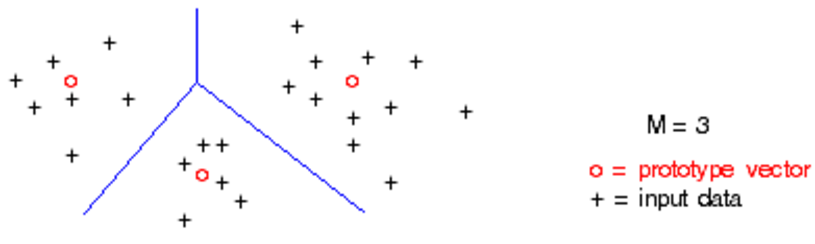
\includegraphics[width=\linewidth]{figures/ch07_vq.pdf}
	\caption{Merkmalsraum als Voronoidiagram: Dargestellt sind die $M=3$ mit $o$ gekennzeichneten Prototypvektoren und die daraus resultierenden Clustergrenzen.}
	\label{fig:ch07_vq}
\end{figure}

\subsection*{Überwachte Vektorquantisierung}
Learning Vector Quantization (LVQ) unterteilt, wie auch VQ, einen Eingaberaum durch eine Menge von Prototypvektoren in Klassen, welche den Eingaberaum möglichst gut wiedergeben. Jedes Element des Eingaberaums soll also einem solchen Vektor (nämlich dem am nächst gelegenen) zugeordnet werden können.
So wird der Eingaberaum in ein \emph{Voronoidiagramm} und damit auch in die besagten diskreten Bereiche unterteilt (siehe Abbildung \ref{fig:ch07_vq}).

Wichtig dabei ist, dass im Voraus die \emph{Anzahl der Klassen}, sowie die \emph{Klassenzugehörigkeit} eines jeden Trainingsbeispiels bekannt sein müssen. Die Klassen müssen dabei nicht disjunkt sein, sie dürfen sich also überlappen.

LVQ arbeitet mit \emph{einschichtigen} Neuronalen Netzen\footnote{Einschichtige NN sind Netze, die aus einer Schicht \emph{aktiver} Neuronen (evtl. mit vorgeschalteten Eingabeneuronen ohne Informationsverarbeitung) bestehen. Diese Neuronen werden oft als \emph{Kohonen-Neuronen} bezeichnet.} und passt die zufällig initialisierten Codebookvektoren durch Trainingsbeispiele so an, dass sie die Trainingsdaten möglichst gut widerspiegeln.



% ----------------------------------------------------------------------
% ----------------------------------------------------------------------
\section*{Training}
Für das Training von LVQ existiert eine Trainingsmenge $P$ mit $|P|$ Trainingsbeispielen, sowie eine Klassenmenge $C$ mit $|C|$ Klassen. Jeder dieser Klassen ist ein Codebookvektor eindeutig zugeordnet. Die Klassenmenge enthält damit $|C|$ Codebookvektoren $C_1, C_2, \ldots, C_{|C|}$.
\begin{hint}{Hinweis!}{lvq-training}
	Möglicherweise können auch mehrere Codebookvektoren für eine Klasse existieren. Das konnte ich nicht genau herausfinden.
	\begin{flushright}\textit{Beni}\end{flushright}
\end{hint}

\begin{hint}{Hinweis!}{prototypvektoren}
	In den folgenden Abbildungen wird ein Eingabemuster anstelle von $p$ mit $X$ und ein Prototypvektor anstelle von $C_i$ mit $W_i$ bezeichnet.
\end{hint}

Die Trainingsbeispiele sind von der Form $(p,c)$. Dabei ist $p \in P$ ein Trainingsmuster und $c \in \{1,2, \ldots, |C|\}$ dessen Klassenzugehörigkeit.

Das LVQ-Lernverfahren besteht grundsätzlich aus den folgenden Schritten:
\begin{itemize}
	\item \emph{Initialisierung} - Die $|C|$ Codebookvektoren werden zufällig im Eingaberaum platziert.
	\item \emph{Trainingsbeispiel} - Ein Trainingsbeispiel $p$ aus der Trainingsmenge $P$ wird gewählt und präsentiert.
	\item \emph{Abstandsmessung} - Der Abstand $||p - C_i||$ aller Codebookvektoren zur Trainingseingabe $p$ wird gemessen.
	\item \emph{Gewinner} - Derjenige Codebookvektor gewinnt, für den gilt:
	\begin{align*}
		\underset{C_i \in C}{min} ||p - C_i||		
	\end{align*}
	\item \emph{Lernvorgang} - Der Lernvorgang findet durch die folgenden Regeln statt:
	\begin{align*}
		\Delta C_i &= \eta(t) \cdot h(p, C_i) \cdot (p-C_i) \\
		C_i(t+1) &= C_i(t) + \Delta C_i
	\end{align*}
	Dabei ist $\eta$, wie gewohnt, die Lernrate und $(p-C_i)$ die Richtung, in die der Codebookvektor verschoben wird.
	Für das Kernstück, die Funktion $h(p, C_i)$, wird eine Fallunterscheidung vorgenommen.
	\begin{itemize}
		\item \emph{Zuweisung richtig} - Der Gewinnervektor ist der Codebookvektor der $p$ zugehörigen Klasse.\\
		In diesem Fall liefert die Funktion $h(p, C_i)$ positive Werte, der Codebookvektor bewegt sich \emph{auf $p$ zu}.
		\item \emph{Zuweisung falsch} - Der Gewinnervektor repräsentiert nicht die Klasse, der $p$ zugehörig ist.\\
		Der Gewinnervektor bewegt sich \emph{von $p$ weg}.
	\end{itemize}
\end{itemize}

Die Funktion $h$ wurde an dieser Stelle nicht genau definiert. Sie unterscheidet sich bei den, im Folgenden aufgeführten Varianten von LVQ: LVQ1, LVQ2, LVQ3, OLVQ.


% ----------------------------------------------------------------------
% ----------------------------------------------------------------------
\section*{LVQ1}
Bei LVQ1 gilt für $h$:
\begin{align*}
	h(p, C_i) =
	\begin{cases}
		+1 \quad \text{wenn } Klasse(C_i) = Klasse(p) \\
		-1 \quad \text{wenn } Klasse(C_i) \ne Klasse(p) \\
	\end{cases}
\end{align*}
\noindent
Die Lernrate $\eta(t)$ kann konstant sein oder mit der Zeit monoton fallen, um Konvergenz zu erzwingen. Es gilt jedoch: $0 < \eta(t) < 1$.
Die Adaption der Prototypvektoren wird in Abbildung \ref{fig:ch07_lvq1} grafisch veranschaulicht.

\begin{figure}[ht!] \centering 
	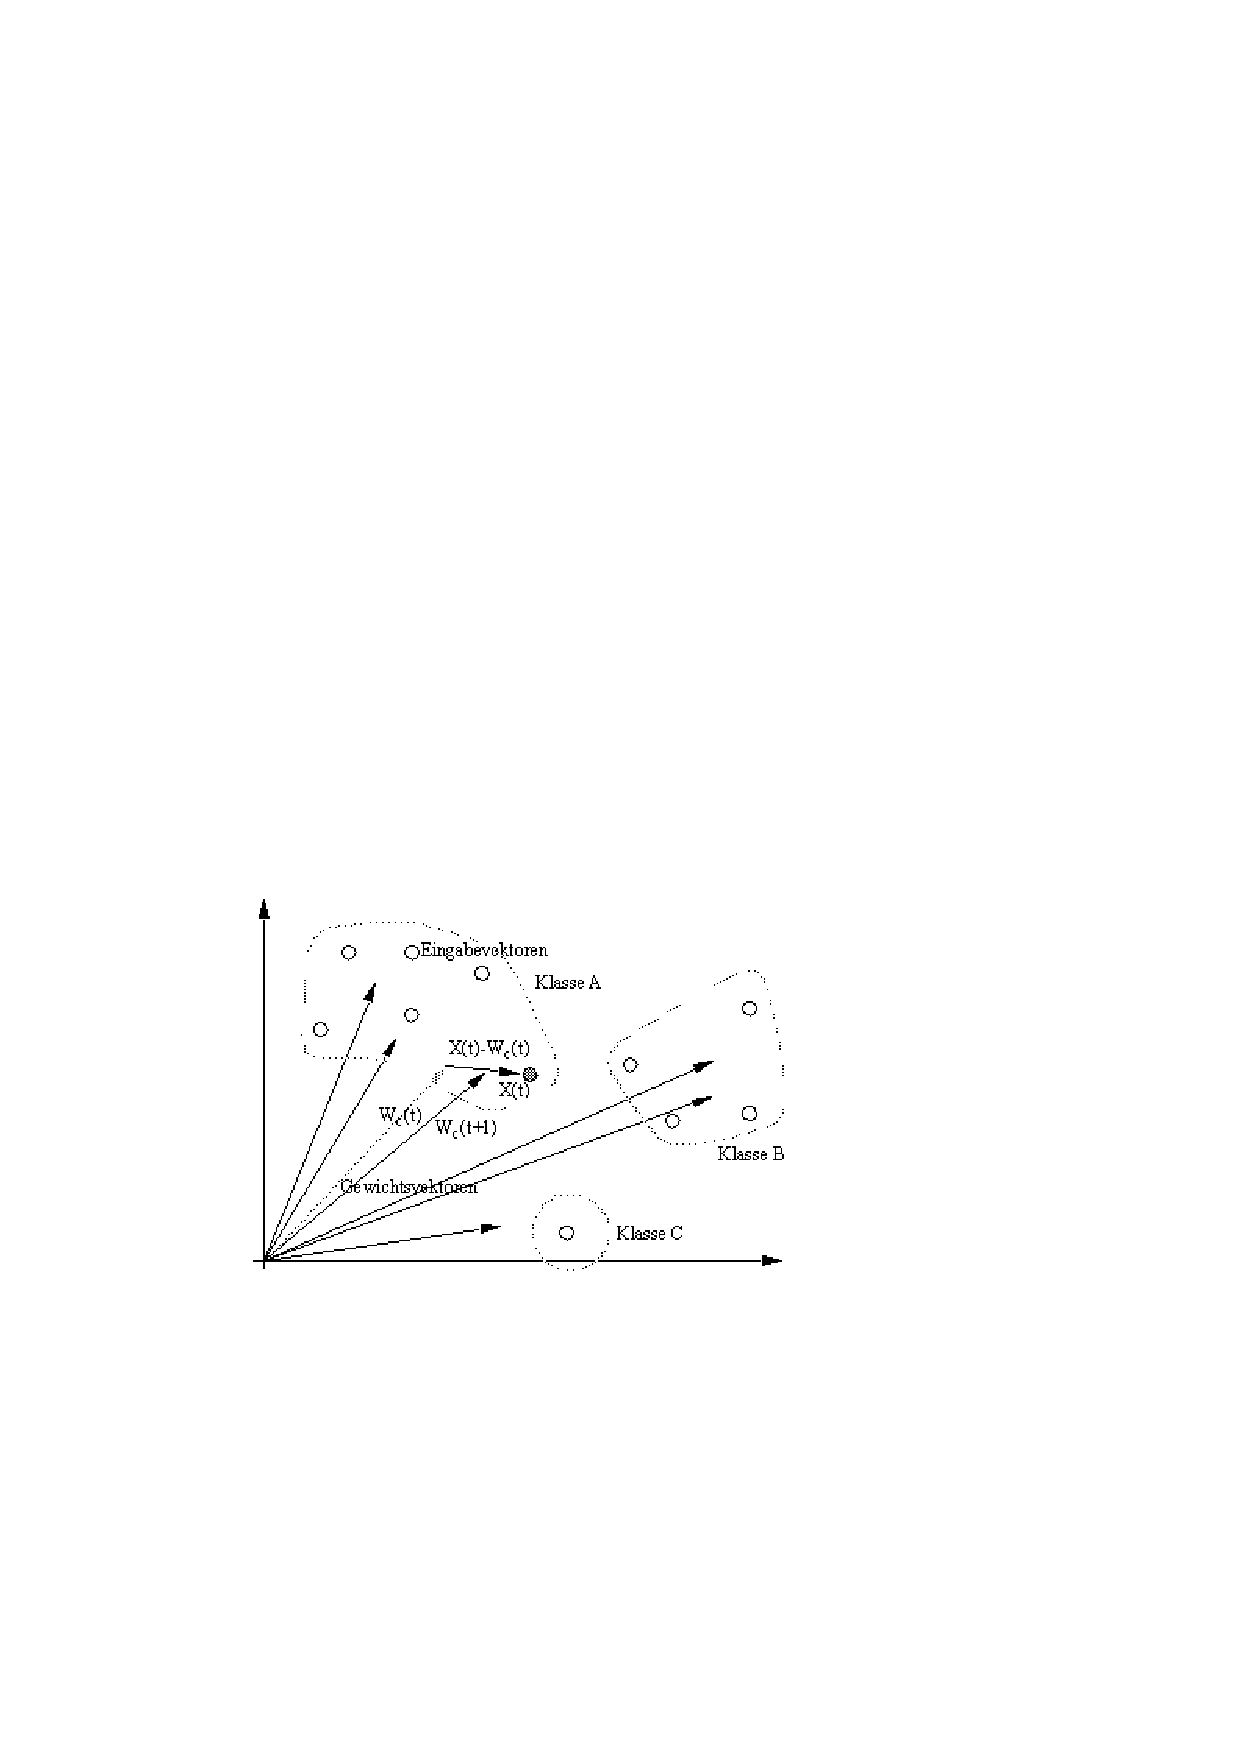
\includegraphics[width=\linewidth]{figures/ch07_lvq1.pdf}
	\caption{Adaption des nächsten Prototypvektors $W_c(t)$ zum Eingabevektor $X(t)$. Hier sind die Eingabevektoren als kleine Kreise, die Prototypvektoren als Pfeile dargestellt. Weiterhin ist hier $Klasse(X) = Klasse(W_c)$.}
	\label{fig:ch07_lvq1}
\end{figure}



% ----------------------------------------------------------------------
% ----------------------------------------------------------------------
\section*{LVQ2.1}
Bei dem Verfahren LVQ2.1 ist die Klassifikation der Eingabe identisch wie bei LVQ1, nur die Modifikation der Prototypvektoren beim Lernen ist anders.
LVQ2.1 sucht \emph{zwei} Prototypvektoren:
\begin{enumerate}
	\item Den \emph{nächsten} Prototypvektor $C_i$ und
	\item Den \emph{übernächsten} Prototypvektor $C_j$.
\end{enumerate}
Dabei findet nur dann eine Adaption der Prototypvektoren statt, wenn folgende Voraussetzungen erfüllt sind:
\begin{itemize}
	\item $Klasse(C_i) \ne Klasse(C_j)$
	\item $Klasse(p) = Klasse(C_i) \vee Klasse(p) = Klasse(C_j)$ 
	\item $p$ liegt in einem "`Fenster"' entlang der Mittelsenkrechten zwischen den beiden Klassen $Klasse(C_i)$ und $Klasse(C_j)$.
\end{itemize}

\subsection*{Das "`Fenster"'}
Wenn man mit $d_i$ und $d_j$ die euklidischen Abstände des Eingabevektors $p$ von den Vektoren $C_i$ und $C_j$ bezeichnet, dann fällt der Eingabevektor $p$ in ein Fenster mit relativer Breite $v$ falls gilt:
\[
	min(\frac{d_i}{d_j}, \frac{d_j}{d_i}) > s
	\quad \text{wobei } s = \frac{1-v}{1+v}
\]
Nach Kohonen sollte die Breite $v$ des relativen Fensters zwischen $0.2$ und $0.3$ betragen. Man beachte, dass dieses "`Fenster"' kein Rechteck ist.
Grafisch kann man sich das wie in Abbildung \ref{fig:ch07_lvq2} gezeigt veranschaulichen. Dort wurde der Wert $v=0.2$ verwendet, wodurch sich $s = \frac{2}{3}$ ergab.

\begin{figure}[ht!] \centering 
	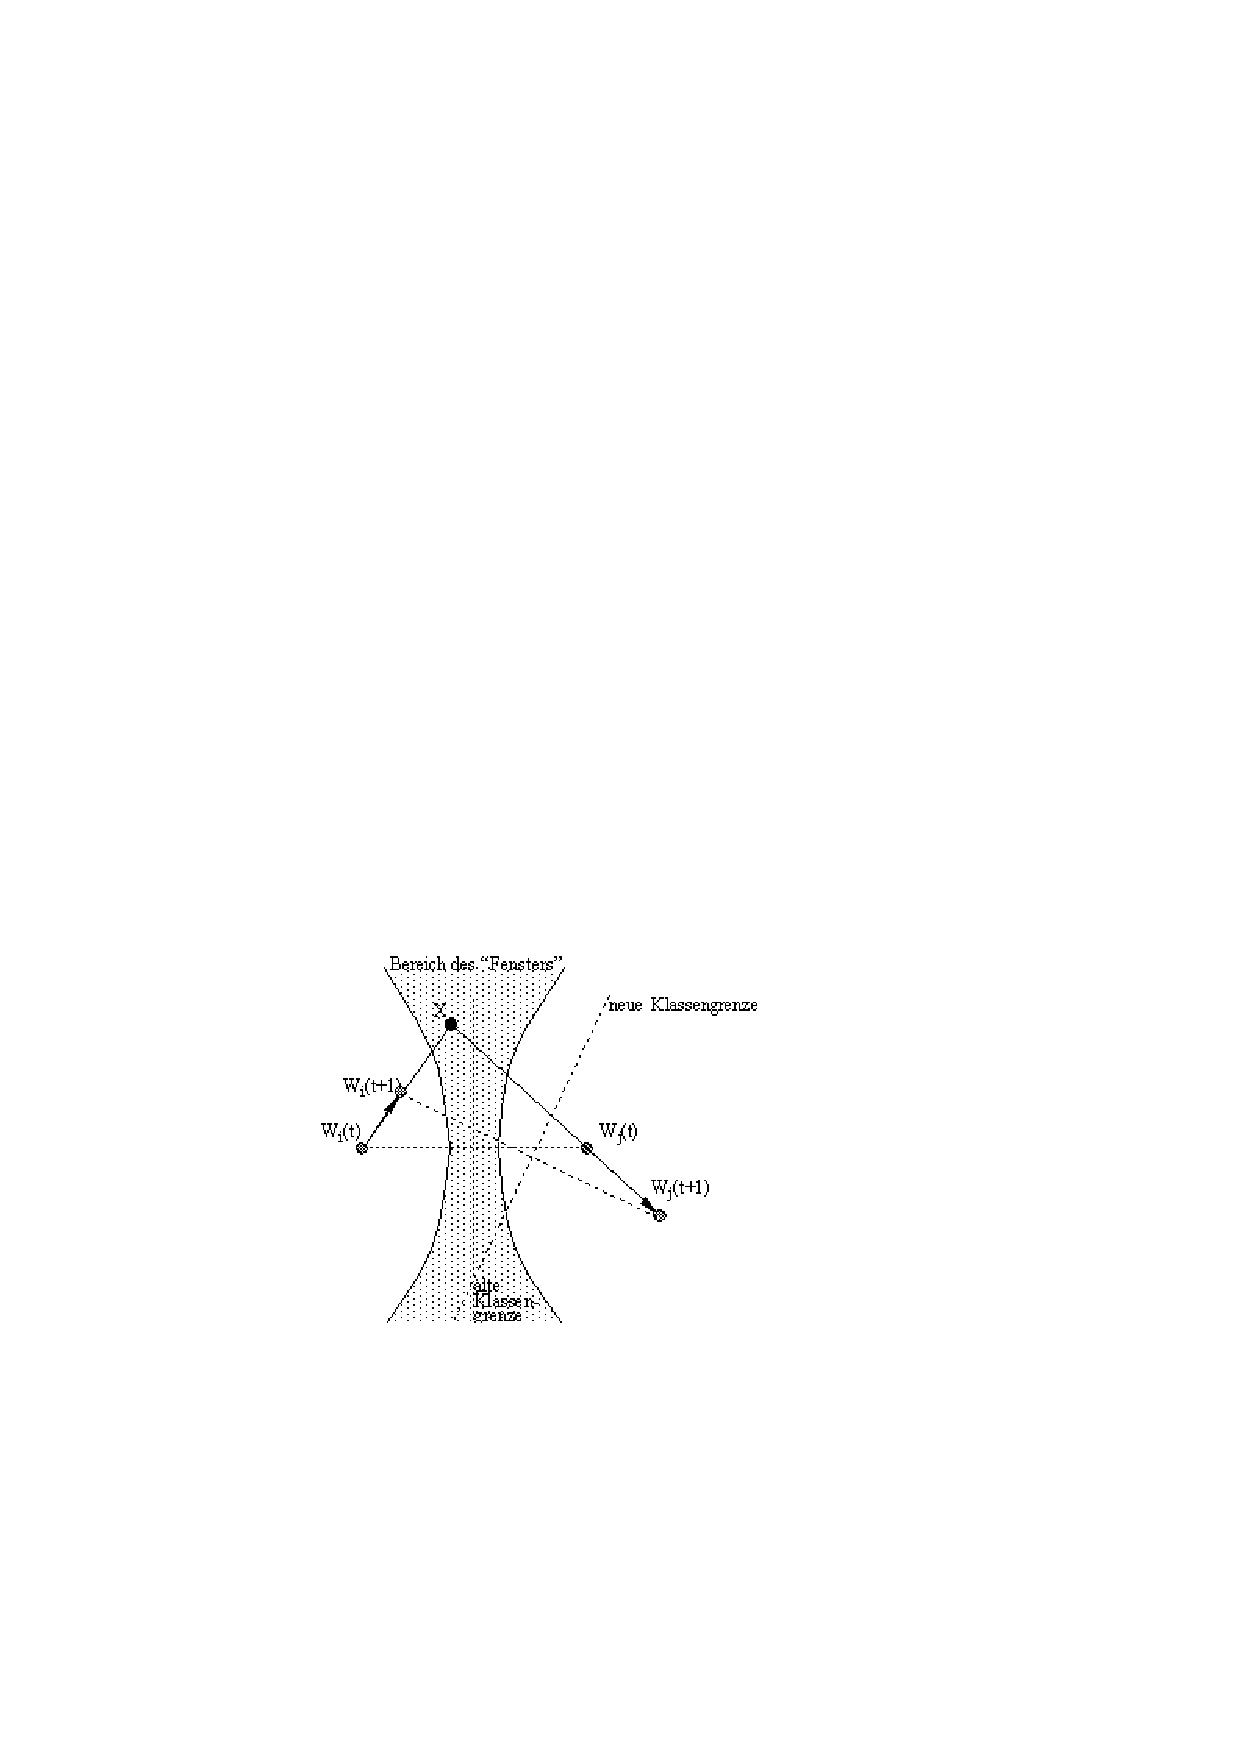
\includegraphics[width=\linewidth]{figures/ch07_lvq2.pdf}
	\caption{Prinzip von LVQ 2.1: Der Prototypvektor $W_i(t)$, dessen Klasse mit der des Musters $X$ übereinstimmt, wird in Richtung des Eingabevektors $X$ verschoben. Der nächste Vektor $W_j(t)$, dessen Klasse \emph{nicht} mit der des Musters $X$ übereinstimmt, wird von $X$ weggeschoben. Dadurch dreht sich die durch die Mittelsenkrechte der Verbindungslinien gebildete Klassengrenze.}
	\label{fig:ch07_lvq2}
\end{figure}
\noindent
Die Formeln für die Anpassung der Prototypvektoren lauten:
\begin{align*}
	C_i(t+1) &= C_i(t) + \eta(t) \Big( p(t) - C_i(t) \Big) \\
	C_j(t+1) &= C_j(t) - \eta(t) \Big( p(t) - C_j(t) \Big)
\end{align*}

Dieses Verfahren modifiziert nur die Grenzflächen der Klassen durch Verschieben der Vektoren, es garantiert jedoch nicht mehr, dass die Dichte
der Vektoren die Verteilungsdichte der Eingabevektoren annähert. Um diesen Mangel wieder zu beheben, wurde LVQ3 entwickelt.


% ----------------------------------------------------------------------
% ----------------------------------------------------------------------
\section*{LVQ3}
Das Verfahren LVQ3 ist eine Erweiterung des Verfahrens LVQ2.1, bei dem zusätzlich zur Änderung der Gewichtsvektoren an einer Klassengrenze die Vektoren $C_i$ und $C_j$ verändert werden, wenn beide der gleichen Klasse wie $X$ angehören.

Für die Anpassung der Prototypvektoren gilt (wie bei LVQ2.1):
\begin{align*}
	C_i(t+1) &= C_i(t) + \eta(t) \Big( p(t) - C_i(t) \Big) \\
	C_j(t+1) &= C_j(t) - \eta(t) \Big( p(t) - C_j(t) \Big)
\end{align*}
wenn die beiden nächsten Vektoren $C_i$ und $C_j$ verschiedenen Klassen angehören, $C_i$ zur gleichen Klasse gehört wie $p$, $C_j$ zu einer anderen Klasse, und $p$ in das "`Fenster"' an der Grenze der beiden Klassen fällt.

Wenn jedoch $C_i$ und $C_j$ der gleichen Klasse wie $p$ angehören, werden - im Gegensatz zu LVQ2.1 - auch beide geändert:
\begin{align*}
	C_i(t+1) &= C_i(t) + e \eta(t) \Big( p(t) - C_i(t) \Big) \\
	C_j(t+1) &= C_j(t) + e \eta(t) \Big( p(t) - C_j(t) \Big)
\end{align*}
Als gute Richtwerte von $e$ gelten Werte zwischen $0.1$ und $0.5$, wobei der Wert für $e$ von der Größe des Fensters abhängt und für engere Fenster besser kleiner zu wählen ist.


% ----------------------------------------------------------------------
% ----------------------------------------------------------------------
\section*{OLVQ1}
Für das Verfahren LVQ1 ist es möglich, die Lernrate für \emph{schnelle Konvergenz} des Verfahrens zu optimieren. Dies führt zum Verfahren OLVQ1. Das optimierte LVQ1 (optimized learning vector quantization, OLVQ1) ist eine Erweiterung von LVQ1, bei der jedem Prototypvektor (Codebookvektor) eine eigene Lernrate $\eta_c(t)$ zugewiesen wird:
\begin{align*}
	C_c(t+1) &= C_c(t) + h(t) \eta_c(t) \Big( p(t) - C_c(t) \Big)\\
	&\text{mit} \\
	\eta_c(t) &= \frac{\eta_c(t-1)}{1 + h(t) \eta_c(t-1)}
\end{align*}
\noindent
Wobei für $h(t)$ gilt:
\[
	h(t) = 
	\begin{cases}
		+1 &\text{wenn } Klasse(C_c) = Klasse(p) \\
		-1 &\text{wenn } Klasse(C_c) \ne Klasse(p)
	\end{cases}
\]

Dies ist die Regel für die optimale Änderung der Lernfaktoren $\eta_c(t)$. Da $\eta_c(t)$ auch anwachsen kann, aber nicht über den Wert $1$ wachsen
darf (andernfalls wird der Vektor nicht zu $p$ hingezogen, sondern über die Verbindungslinie hinter $p$ hinaus bewegt), muss sichergestellt werden, dass $\eta_c(t)$ nicht über $1$ anwächst. 



% ----------------------------------------------------------------------
% ----------------------------------------------------------------------
\section*{Unterschiede}
LVQ3 ist stabiler als LVQ2.1, ein fortlaufendes Lernen verändert optimal eingestellte Gewichtsvektoren nicht mehr.
Die beiden Verfahren LVQ1 und LVQ3 passen die Lage der Codebookvektoren der Verteilung der Eingabevektoren an, während LVQ2.1 nur die relativen Entfernungen der Codebookvektoren von der Grenzlinie zwischen den Klassen optimiert. Dies garantiert nicht, dass diese Vektoren optimal platziert sind, um die Form der Klassengrenze anzunähern. LVQ2.1 sollte daher in erster Linie zur schärferen Klassentrennung mit einer kleinen Lernrate und einer relativ kleinen Zahl von Lernschritten verwendet werden.


% ----------------------------------------------------------------------
% ----------------------------------------------------------------------
\section*{Bemerkungen}
Die Genauigkeit, mit der eine Klassifikationsaufgabe mit LVQ gelöst werden kann, hängt von einer Reihe von Faktoren ab:

\begin{itemize}
	\item der Zahl der verfügbaren Codebookvektoren für jede Klasse
	\item der Initialisierung der Codebookvektoren
	\item dem verwendeten Lernalgorithmus
	\item der richtigen Lernrate für die einzelnen Schritte
	\item einem richtigen Abbruchkriterium zur Terminierung des Lernens
\end{itemize}

\subsection*{Codebookvektoren}
Für viele Anwendungen ist es ausreichend, mit einer gleichen Anzahl von Codebookvektoren (Neuronen) für jede Klasse zu arbeiten, selbst wenn die a-priori-Wahrscheinlichkeiten der Zugehörigkeit der Eingabemuster zu den einzelnen Klassen stark differieren.
Eine obere Grenze für die Gesamtzahl der Codebookvektoren ist zumeist die begrenzte Rechenzeit beim Training oder bei der Klassifikation in der Arbeitsphase.

Für die Anfangsinitialisierung der Codebookvektoren wählt man oft als
Initialwerte Vektoren aus den Trainingsdaten aus. Damit verhindert man, dass Codebookvektoren Initialwerte besitzen, die weit entfernt von den Werten der Trainingsmuster sind. Diese Vektoren wären dann nämlich nie die nächsten Nachbarn zu den Eingabevektoren und würden nie verändert werden.

\subsection*{Training}
Die Grenzen der Erkennungsgenauigkeit werden nach einer Zahl von Lernschritten erreicht, die der 30- bis 50-fachen Zahl der Codebookvektoren entspricht, d.h. jedes Neuron wird im Mittel zwischen 30 und 50 Mal verändert.

Läßt man die LVQ-Verfahren zu lange lernen, so tritt oft der Effekt des \emph{Übertrainierens} auf.
Der Trainingsvorgang sollte daher nicht unbegrenzt fortgeführt werden, sondern nach einer Schrittzahl, die ca. der 50- bis 200-fachen Zahl der Codebookvektoren entspricht (abhängig von Algorithmus und Lernrate), abgebrochen werden. Die Schrittzahl ist natürlich auch abhängig von den Eingabevektoren und damit vom Problem.

